%!TEX root = ./../../springer-mono-format/book.tex
%!TEX root = ./../../thesis-trier.tex

Here,  we introduce several situations and problems
which can be modeled using synchronizing automata:
a problem from coding theory in \cref{intro:sec:examples:communication},
a puzzle from Ashby in \cref{intro:sec:examples:puzzle},
a conveyor belt and part orienter design problem in \cref{intro:sec:examples:partorienters},
and a maze orientation problem in \cref{intro:sec:examples:maze}.

\subsection{Error-Prone Communication Channels}
\label{intro:sec:examples:communication}

Suppose five symbols $e,h,l,o,r$ are encoded by five binary sequences $00$, $01$, $10$, $110$,
and $111$, respectively, see \cref{fig:intro:encoding}. This coding scheme is taken from Neumann~\cite{neumann71}. 

\begin{figure}[t]
	\centering
	\begin{subfigure}[b]{.38\textwidth}
		\centering
		\[
		\begin{array}{c|c}
			\text{Symbol} & \text{Binary Encoding} \\ \hline 
			e & 00 \\
			h & 01 \\
			l & 10 \\
			o & 110 \\
			r & 111
		\end{array} 
		\]
		\caption{Encoding of source symbols.}
		\label{intro:fig:decoder:code}
	\end{subfigure}%
	\hfill
	\begin{subfigure}[b]{0.6\textwidth}
		\centering
		\begin{tikzpicture}[shorten >=1pt,node distance=1.5cm and 1cm,on grid,auto,font=\sffamily] 
			\node (eps)  {$\varepsilon$};
			\node (0) [xshift=-0.7cm,  below left=of eps]  {$0$};
			\node (1) [xshift=0.7cm, below right=of eps] {$1$};
			\node (11) [below right=of 1]  {$11$};
			\node (00)  [below left = of 0]   {$00$};
			\node (01)  [below right = of 0]  {$01$};
			\node (110) [below left = of 11]  {$110$};
			\node (111) [below right = of 11] {$111$};
			\node (10)  [below left = of 1] {$10$};
			
			\path[->] (eps) edge [dashed] node {} (0)
			(eps) edge node {} (1)
			(1)   edge node {} (11)
			(0)   edge [dashed] node {} (00)
			(0)   edge node {} (01)
			(11)  edge [dashed] node {} (110)
			(11)  edge node {} (111)
			(1)   edge [dashed] node {} (10);
			
			\node (e) [yshift=0.9cm, below = of 00] {$e$};
			\node (h) [yshift=0.9cm, below = of 01] {$h$};
			\node (l) [yshift=0.9cm, below = of 10] {$l$};
			\node (o) [yshift=0.9cm, below = of 110] {$o$};
			\node (r) [yshift=0.9cm, below = of 111] {$r$};
		\end{tikzpicture}
		\caption{Decision tree to decode symbols for binary inputs where dashed and solid branches correspond to $0$ and $1$, respectively.}
		\label{fig:tree-encoding}
	\end{subfigure}
	\caption{Encoding of five symbols $e$, $h$, $l$, $o$, and~$r$  by binary sequences.}
	\label{fig:intro:encoding}
\end{figure}

When transmitting a message using this code, is it possible to recover from a loss of synchronization between the sender (encoder) and receiver (decoder) caused by channel errors?
For example, suppose the sender wants to transmit ``hello'' 
to the receiver, which corresponds to the bit sequence ``$01\ 00\ 10\ 10\ 110$''. However, after sending the first three bits, the sender is uncertain whether they were received correctly.

On the receiving end, a stream of code words can be decoded with the help of the automaton 
shown in \cref{intro:subfig:decoder},
which starts in the state~$q_{\varepsilon}$ and reflects different states of the receiver.
A path starting in~$q_{\varepsilon}$ and going back to~$q_{\varepsilon}$
corresponds to a received code word, 
where the transition leading into~$q_{\varepsilon}$
indicates which code word was received.
For example, when reading ``$01\ 00\ 10\ 10\ 110$'', starting from $q_{\varepsilon}$,
the transitions returning to $q_{\varepsilon}$ indicate the sequence ``hello'' in that order. 

\begin{figure}[ht]
	\centering
	\begin{subfigure}[b]{.6\textwidth}
		\centering
			\begin{tikzpicture}[shorten >=1pt,node distance=3cm,on grid,auto,font=\sffamily] 
				\node[state,blur shadow,fill={rgb:black,0.4;white,10}] (eps)  {$q_{\varepsilon}$};
				\node[state,blur shadow,fill={rgb:black,0.4;white,10}] (0) [below left=of eps]  {$q_{0}$};
				\node[state,blur shadow,fill={rgb:black,0.4;white,10}] (1) [xshift=-0.3cm, yshift=0.3cm, below right=of eps] {$q_{1}$};
				\node[state,blur shadow,fill={rgb:black,0.4;white,10}] (11) [xshift=-0.7cm, yshift=0.7cm,below right=of 1]  {$q_{11}$};
				
				\path[->] (eps) edge [dashed] node {} (0)
				(eps) edge node {} (1)
				(1)   edge node {} (11)
				(0)   edge [dashed,out=90,in=190, below, pos=.7] node {$e$} (eps)
				(0)   edge [out=130,in=150,pos=.7] node {$h$} (eps)
				(1)   edge [dashed,out=180, in=280, above] node {$l$} (eps)
				(11)  edge [dashed,out=190, in=270, pos=.8] node {$o$} (eps)
				(11)  edge [out=80, in=0, above, pos=0.8] node {$r$} (eps);
		\end{tikzpicture}
		\caption{Starting from $q_{\varepsilon}$, each return to $q_{\varepsilon}$ 
			corresponds to the decoding of one code word; the label on the return transition indicates the decoded source symbol.
		}
	\label{intro:subfig:decoder}	
\end{subfigure}%
\hfill
\begin{subfigure}[b]{0.35\textwidth}
	\centering
	\[
	\begin{array}{l|lllll}
		& 0 & 1 & 1 & 0 \\ \hline       
		q_{\varepsilon} & q_0 & q_{\varepsilon} & q_1 & q_{\varepsilon}  \\
		q_{0}           & q_{\varepsilon} & q_{1} & q_{11} & q_{\varepsilon} \\
		q_1             & q_{\varepsilon} & q_1   & q_{11} & q_{\varepsilon} \\
		q_{11}          & q_{\varepsilon} & q_1   & q_{11} & q_{\varepsilon}
	\end{array}
	\]
	\caption{The state transitions for the input sequence $0110$ starting from each state.}
	\label{intro:fig:decoder:syncsequence}
\end{subfigure}
\caption[Introductory decoder automaton]{Decoder automaton (left) 
	for the code from \cref{fig:intro:encoding}
	where dashed (resp. solid) transitions represent input symbol $0$ (resp. $1$)
	with the synchronizing word $0110$ (right).} 
\label{intro:fig:decoder}	
\end{figure}

Now suppose that the current state of the decoder automaton is unknown. This raises the following question.

\smallskip
\begin{center}
	\fbox{%
		\begin{minipage}{29em}
			Can the sender transmit a sequence of bits that guarantees the receiver
			is brought to the well-defined state $q_{\varepsilon}$ in \cref{intro:subfig:decoder},
			from which it can correctly decode the next code word?
		\end{minipage}
	}
\end{center}
\smallskip

The answer is positive: as shown in \cref{intro:fig:decoder:syncsequence},
reading the sequence~$0110$ from any state of the automaton leads to $q_{\varepsilon}$.
Thus, by transmitting~$0110$, the sender can reset the receiver in case it has lost synchronization 
with the stream of code words due to errors, ensuring correct decoding of subsequent bits.

Applied to the situation above, where the sender wants to transmit ``hello'' but is unsure
whether the first three bits were transmitted correctly, the sender can send the message
\[
\underbrace{010}_{\text{uncertain bits}}
0110\,01\,00\,10\,10\,110.
\]

After reading “$010\ 0110$”,
the automaton is in the state $q_{\varepsilon}$, from which it can correctly decode the
next code word.

\subsection{The Haunted Mansion} 
\label{intro:sec:examples:puzzle}
	
Ashby~\cite{ashby_56} presented the following puzzle. A mansion is haunted
by two ghostly noises, Singing and Laughter. 
Each of the noises can independently be either on or off, and they can be influenced
by two possible actions, organ playing or burning incense, according
to the following scheme described by Ashby~\cite[pp.~60--61]{ashby_56}.

\begin{quote} 
The Singing, in the succeeding minute, will go on as it was during the preceding minute (sounding
or silent) unless there was organ-playing with no Laughter, in which case it will change to the opposite (sounding
to silent, or vice versa).

As for the Laughter, if there was incense burning, then it will sound or not according as the Singing was sounding
or not (so that the Laughter copies the Singing a minute later).
If however there was no incense burning, the Laughter will do the opposite of what the Singing did. 
\end{quote} 

The puzzle asks for a sequence of actions that silences both noises when they are both active. However, more is possible: as we shall see, there exists a sequence of actions that leads to both noises becoming silent in every possible situation.

\IN{Ashby's ghost taming automaton}
\begin{figure}[htb]
\centering
\scalebox{0.9}{
\begin{tikzpicture}[
	node distance=14em and 14em,
	on grid,
	auto,
	font=\sffamily,
	>=Stealth,
	shorten >=1pt,
	semithick
	]
	
	\node[state] (00) {$(\overline S, \overline L)$}; 
	\node[state] (01) [right=of 00] {$(\overline S, L)$};
	\node[state] (10) [below=of 01] {$(S, \overline L)$};
	\node[state] (11) [left=of 10] {$(S, L)$};
	
	\path
	(00) edge [loop left] node {$a_{\overline O B}$} (00)
	(00) edge [bend left=11] node {$a_{\overline O \overline B}$} (01)
	(00) edge [bend left=11] node {$a_{O B}$} (10)
	(00) edge [bend right=11] node[left] {$a_{O \overline B}$} (11)
	
	(01) edge [loop right] node {$a_{O\overline B}, a_{\overline O \overline B}$} (01)
	(01) edge [bend left=11] node {$a_{OB}, a_{\overline O B}$} (00)
	
	(10) edge [loop right] node {$a_{\overline O\overline B}$} (10)
	(10) edge [bend left=11] node {$a_{\overline O B}$} (11)
	(10) edge [bend left=11] node {$a_{O \overline B}$} (00)
	(10) edge [bend right=11] node[right] {$a_{OB}$} (01)
	
	(11) edge [loop left] node {$a_{\overline O B}, a_{OB}$} (11)
	(11) edge [bend left=15] node {$a_{O \overline B}, a_{\overline O \overline B}$} (10);
\end{tikzpicture}
}
\caption[Ashby's ghost taming automaton]{Ashby's ghost taming automaton. 
	The word $a_{\overline O \overline B} a_{O \overline B} a_{\overline O  B}$	is synchronizing.}
\label{intro:fig:ashby}
\end{figure} 

We can model the situation 
by an automaton $\semiautomat{A}{Q}{\Sigma}{\delta}$ with
state set 
\[
Q = \{ (S, L), (\overline S, L), (\overline S, \overline L), (S, \overline L) \},
\]
where $S$ and $\overline S$ represent the presence and absence of singing, respectively, 
and similarly for $L$ and $\overline L$ with laughter.
Furthermore, the input alphabet is 
$ \Sigma = \{ a_{OB}, a_{\overline O B}, a_{\overline O \overline B}, a_{O \overline B}\}
$
where the symbols represent the four possible combinations of playing the organ~($O$), 
not playing organ ($\overline O$),
burning incense ($B$), or not burning incense~($\overline B$).
The transitions are given as in \cref{intro:fig:ashby}.

The word $a_{\overline O \overline B} a_{O \overline B} a_{\overline O  B}$
is a synchronizing word ending in the synchronizing state $(\overline S, \overline L)$.
Hence, by executing the corresponding actions, the ghosts end up silent regardless of their current behavior.
As pointed out by Volkov~\cite{DBLP:conf/lata/Volkov08}, this seems to be the first publication in which a synchronizing automaton occurs. However, Ashby did not comment on the existence of a sequence that silences both ghosts under all circumstances.

\subsection{Part Orienters} 
\label{intro:sec:examples:partorienters}

Suppose that, at the end of an assembly line, square-shaped components with a small square inset on one side (see~\cref{intro:fig:part}) must arrive with the inset on the left side (Ananichev and Volkov~\cite{AnanichevVolkov04}; see also~\cite{DBLP:journals/eswa/PodolakRSZ18,DBLP:conf/lata/Volkov08,Volkov22}).
For simplicity, we assume that there are only four possible orientations, shown in \cref{intro:fig:parts-orientations}.
As the components move along the assembly line from left to right, they encounter two kinds of obstacles: high and low. A high obstacle always rotates a component by 90-degree
counterclockwise. A low obstacle rotates the component in the same way only when the inset is on the top side, since only in this orientation does the obstacle touch the component.
Can one place a sequence of obstacles along the assembly line such that, regardless of the initial orientation, the final orientation always has the inset on the left side?

\begin{figure}[ht]
\centering
\begin{subfigure}[t]{0.4\textwidth}
	\centering
	
\includegraphics[width=0.32\textwidth]{../part1/sync/detail.png}
	\caption{A polygonal component.}
	\label{intro:fig:part}
\end{subfigure}\hfill%
\begin{subfigure}[t]{0.45\textwidth}
	\centering

	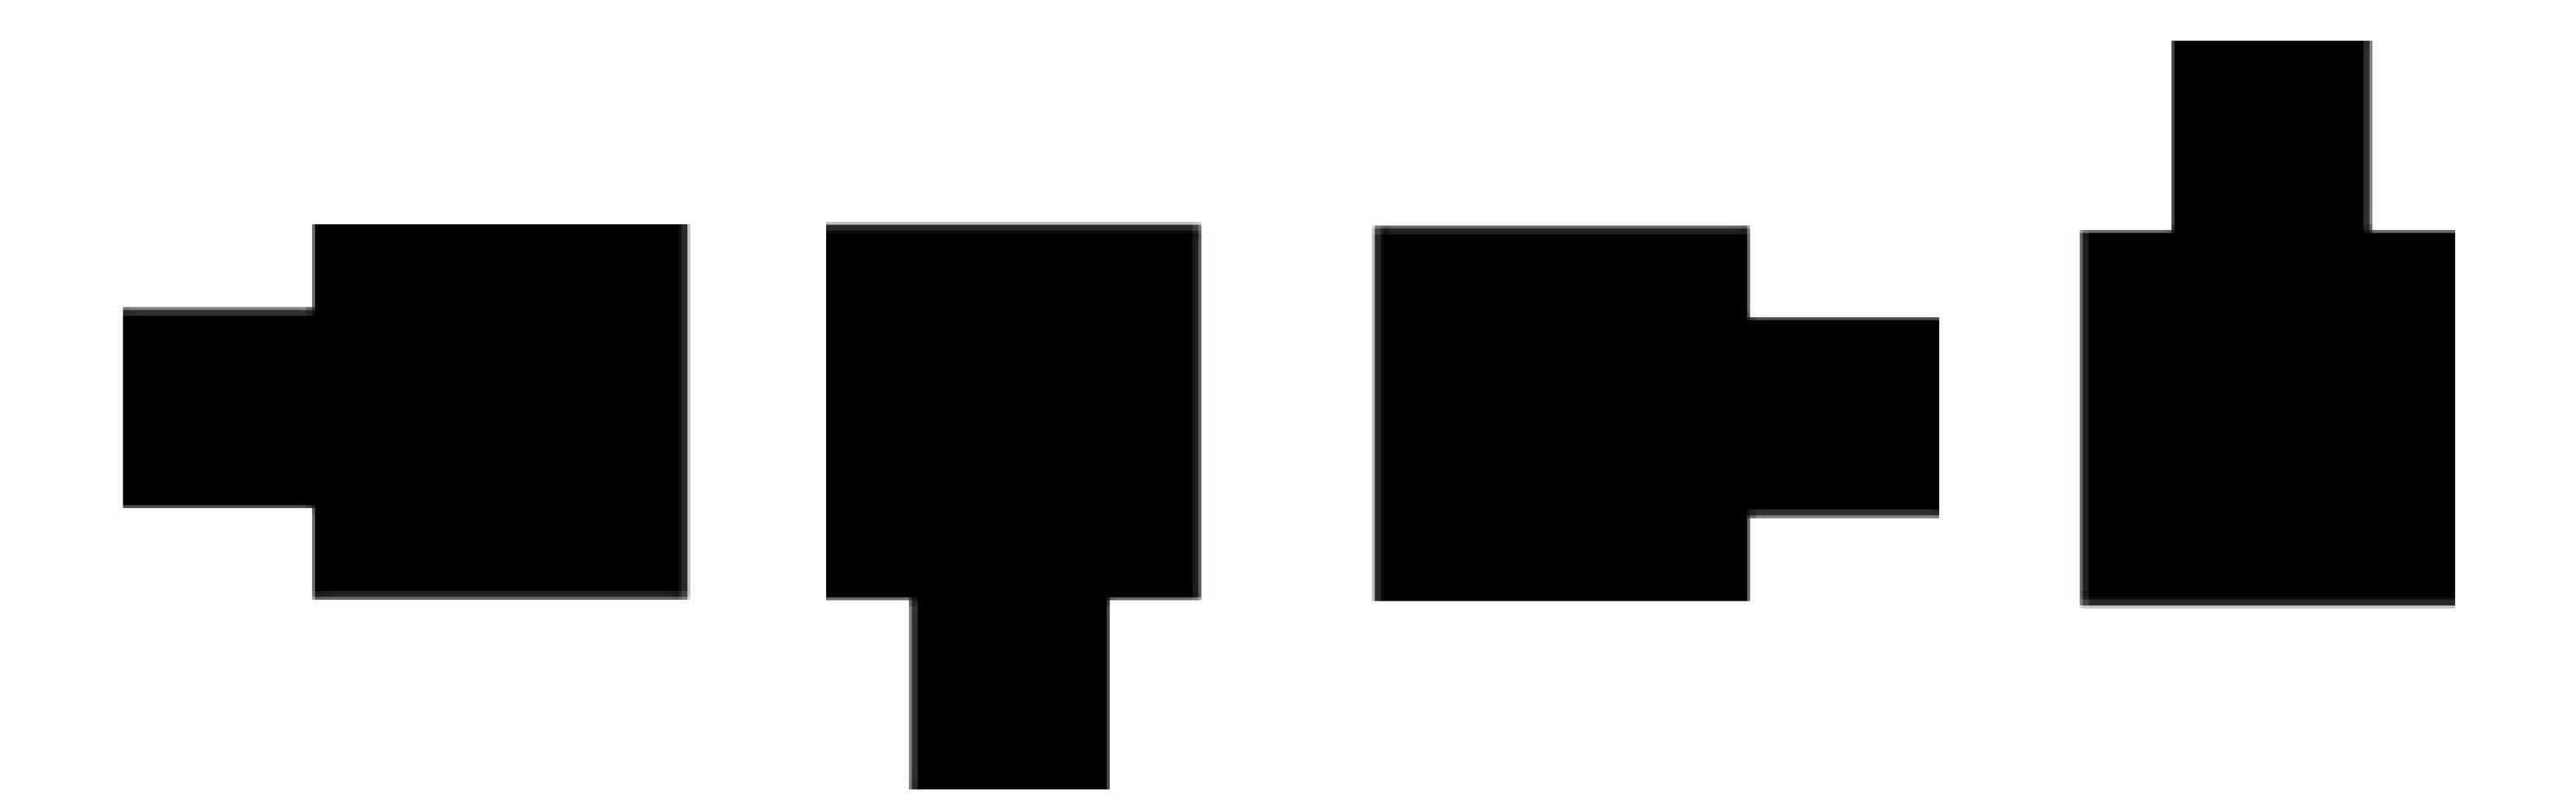
\includegraphics[width=1\textwidth]{../part1/sync/fourorient.png}
	\caption{The four possible orientations.} 
	\label{intro:fig:parts-orientations}
\end{subfigure}
\caption[A polygonal component and its possible orientations]{A polygonal component 
and its possible orientations on an assembly line.} 
\end{figure} 

Taking the four possible orientations as the states of an automaton, the effects of the two types of obstacles can be modeled by two input letters, as illustrated on the left-hand side of \cref{intro:fig:part-orient-solution}. 
As the reader might notice, this construction yields, in essence, the same automaton as the one given earlier in \cref{intro:fig:cernyfour}.
The original problem reduces to determining whether this automaton admits a synchronizing word. One possible synchronizing sequence is low, high, high, high, low, high, high, high, low.
In the case where a component arrives with its insert oriented to the left, the effect of this sequence is shown on the right-hand side of \cref{intro:fig:part-orient-solution}.

\begin{figure}[h]
\centering
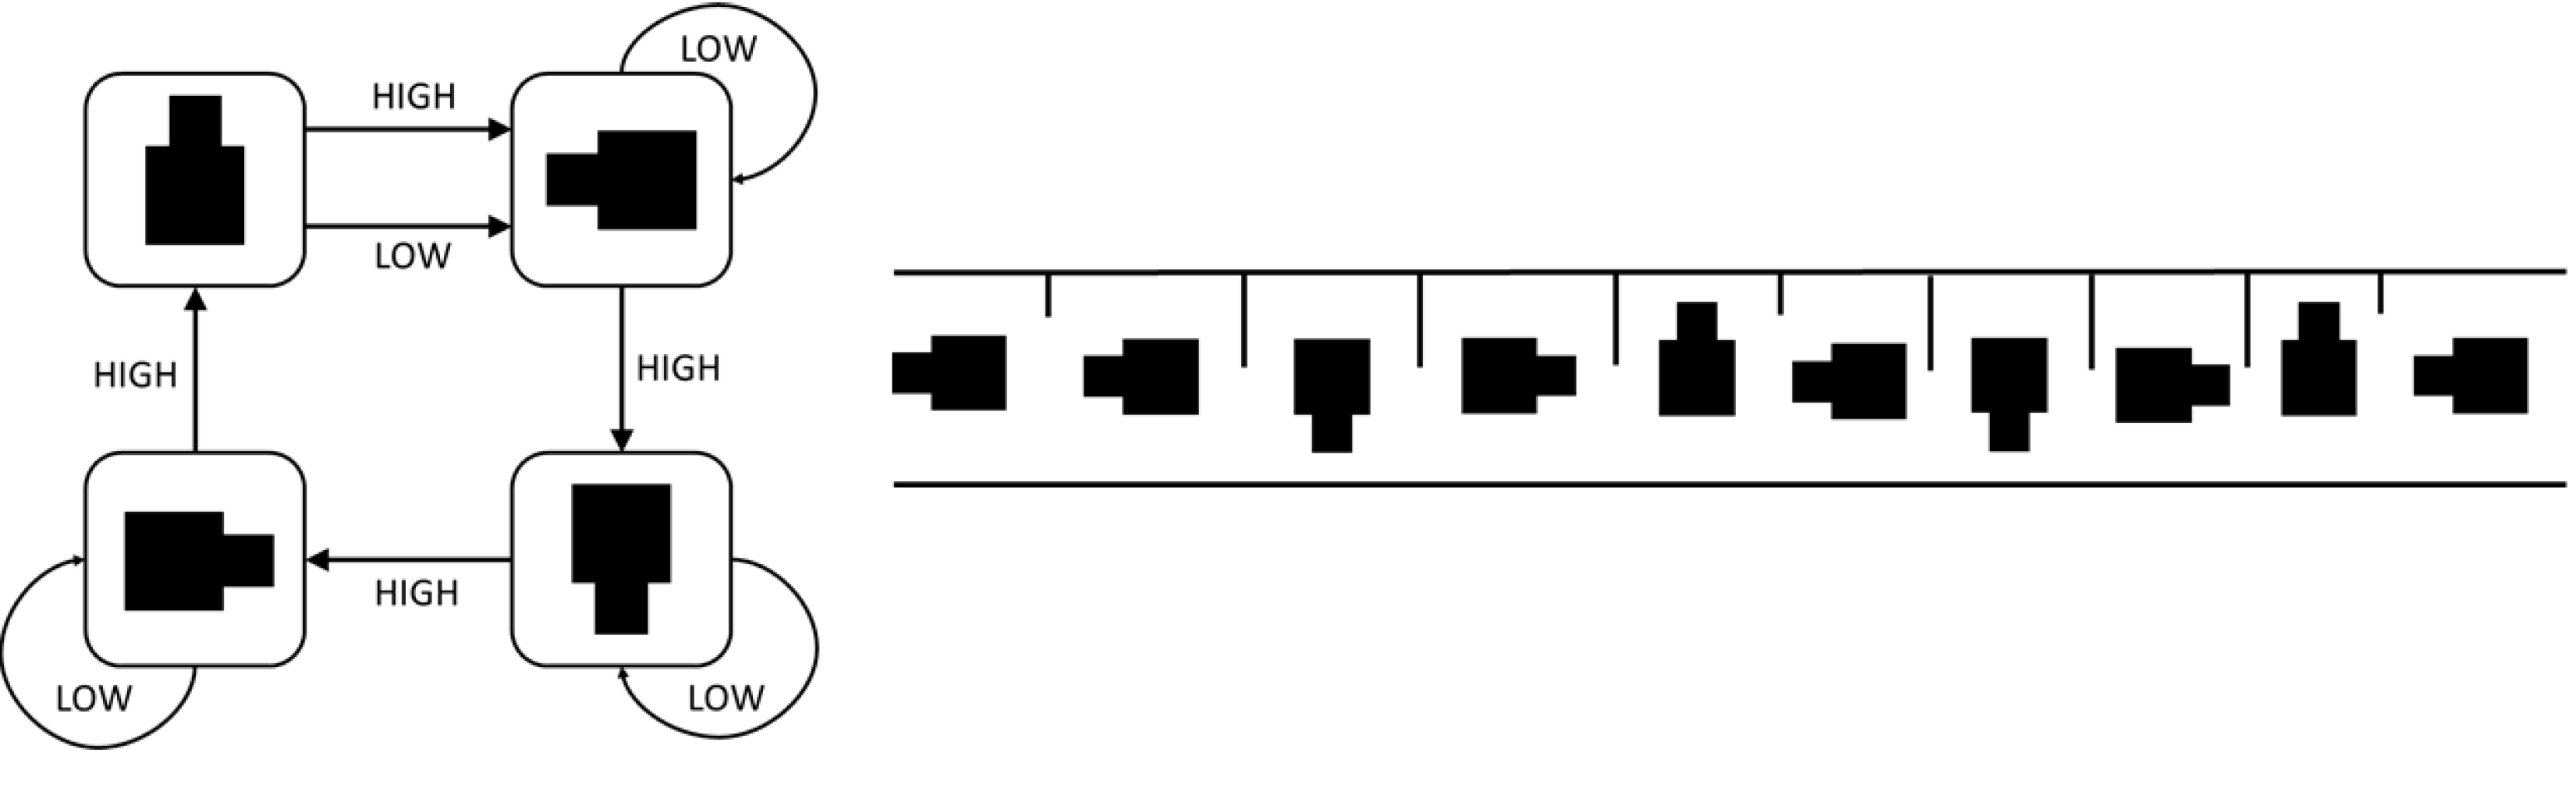
\includegraphics[width=\textwidth]{../part1/sync/part-orienter.png}
\caption[Part orienter problem modeled as a finite automaton]{Left: The part orienter problem modeled as a finite automaton.
	Right: Sequence of effects on one component moving from left to right.		
	Image taken from Podolak et al.~\cite{DBLP:journals/eswa/PodolakRSZ18}. } 
\label{intro:fig:part-orient-solution}	
\end{figure} 

The above scheme works without the use of sensors and does not require any observer or external mechanism to orient the parts. Employing sensorless methods for part orientation is often preferable to using more complicated machinery because of their robustness, simplicity, and ease of maintenance.
In another sensorless approach to part feeding, parts are placed on a vibrating surface and must pass certain obstacles. Such orientation schemes have apparently been employed since the mid-20th century; see~\cite{Sadasivam2015} for a survey on vibratory  part feeders. Sensorless methods for orienting parts without vibrating surfaces were first described by Erdmann and Mason~\cite{DBLP:journals/trob/ErdmannM88}, who simplified and mathematically analyzed a mechanical device originally introduced by Grossman and Blasgen~\cite{DBLP:journals/tsmc/GrossmanB75}.

The first author to investigate the computational complexity of designing sensorless part orienters was Natarajan~\cite{DBLP:conf/focs/Natarajan86,DBLP:journals/ijrr/Natarajan89}. He studied the engineering problem of orienting polygonal objects on conveyor belts using simple, robust, and sensorless methods based on mechanical contact points installed along the belt. Mathematically, he modeled this problem both as a pebbling game and as the problem of finding a sequence of functions from a given set that realizes a constant function. He noted (without proof) 
that a generalization of the latter formulation is \PSPACE-complete and gave polynomial-time algorithms for several variants of these problems.

Natarajan's algorithmic approach to part orienting stimulated substantial
further research in this area. For example,
Goldberg~\cite{DBLP:journals/algorithmica/Goldberg93} introduced a scheme
that orients parts by squeezing them with parallel-jaw grippers and gave a
polynomial-time algorithm for designing a sequence of squeezes that orients
any part, conjecturing that a linear number of squeezes always suffices.
Chen and Ierardi~\cite{DBLP:journals/algorithmica/ChenI95} later confirmed
this conjecture.

Eppstein~\cite{Eppstein90} observed the connection to synchronizing automata previously studied in automata theory, characterized the class of automata investigated by Natarajan~\cite{DBLP:conf/focs/Natarajan86}, and improved Natarajan's algorithms. In this sense, 
synchronizing automata emerged independently in the mechanical engineering literature.
Part orienting as a motivating example for synchronizing automata was later popularized by Ananichev and Volkov~\cite{AnanichevVolkov04,DBLP:journals/tcs/AnanichevV04}; see also the widely cited survey~\cite{DBLP:conf/lata/Volkov08}.

\subsection{Lost in a Maze} 
\label{intro:sec:examples:maze}

Imagine a maze in which every junction has exactly $k$ outgoing corridors
and all junctions look alike, so that a visitor can never tell where they
currently are. The corridors leaving a junction are to be marked with $k$
distinct colors, one color per corridor, and a visitor who is told a
sequence of colors follows the corresponding corridors one after the other.
The task of whoever installs the signs is the following.

\smallskip
\begin{center}
	\fbox{%
		\begin{minipage}{0.9\linewidth}%{\dimexpr\linewidth-2\fboxsep-2\fboxrule\relax}
			Can the corridors be colored so that some sequence of colors
			leads every visitor to one and the same junction, no matter
			where in the maze they started?
		\end{minipage}
	}
\end{center}
\smallskip

Such a sequence does not point at the exit directly; it brings all visitors
to a common junction, and from there a single fixed route takes them out.
Coloring the corridors turns the maze into a deterministic finite automaton:
the junctions are the states, the colors form an alphabet of size $k$, and
a corridor colored~$a$ from junction~$p$ to junction~$q$ gives the
transition $\delta(p,a) = q$. The question above then asks whether the
corridors admit a coloring for which the resulting automaton is
synchronizing.

Not every maze does. If, for instance, the junctions can be split into two
groups such that every corridor leads from one group to the other, then two
visitors starting in different groups stay in different groups forever,
whatever the coloring and whatever sequence they are given. Ruling out
obstructions of this kind is in fact enough: the \emph{road coloring
	theorem}, conjectured by Adler, Goodwyn, and Weiss~\cite{adler77} and proved
by Trahtman~\cite{trahtman09} some thirty years later, states that a
synchronizing coloring exists if and only if the maze is strongly connected
and the lengths of its closed walks have greatest common divisor one.
\IN{road coloring theorem}
\IN{road coloring problem|see{road coloring theorem}}